\svnid{$Id: ribbon_scripting.tex 1 2015-10-01 14:42:25Z rodriqu_dd $}

\subsection{Scripting}\label{ssec:scriptingeditorribbon}

When you open the scripting editor in deltashell, a Scripting \menu{ribbon} category will appear. This ribbon has the following additional options (see also \Fref{Fig:RibbonScripting}), which are described in Table \ref{tab:RibbonScripting}:
%
\begin{figure}[H]
\centering
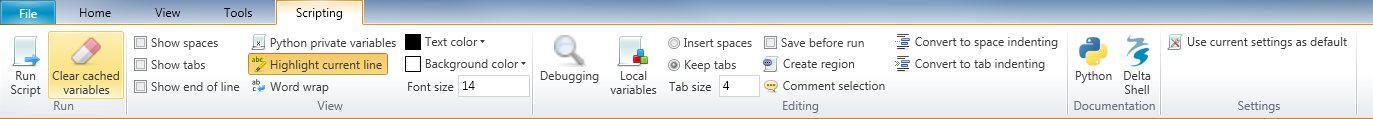
\includegraphics[width=\textwidth]{figures/Ribbon.png}
\caption{The scripting \menu{ribbon} within deltashell.}
\label{Fig:RibbonScripting}
\end{figure}

\begin{longtable}{|p{0.3\textwidth}|p{0.64\textwidth}|}
    \caption{Functions and their descriptions within the scripting \menu{ribbon} of deltashell.\label{tab:RibbonScripting}
} \\
    \hline
    \STRUT \textbf{Function} & \textbf{Description} \\
    [1ex] \hline
\endhead
\hline
\endfoot
    Run script & Executes the selected text. If no text is selected then it will execute the entire script \\
    Clear cached variables & Clears all variables and loaded libraries from memory \\
    Debugging & Enables/Disables the debug option. When enabled you can add breakpoint to the code (using \key{F9} or clicking in the margin) and the code will stop at this point before executing the statement (use F10 (step over) or F11 (step into) for a more step by step approach) \\
    Python variables & Show or hide python variables (like \_var\_) in code completion \\
    Insert spaces/tabs & Determines if spaces or tab characters are added when pressing tab \\
    Tab size & Sets the number of spaces that are considered equal to a tab character \\
    Save before run & Saves the changes to the file before running \\
    Create region & Creates a new region surrounding the selected text \\
    Comment selection & Comments out the selected text \\
    Convert to space indenting & Converts all tab characters in the script to spaces. The number of spaces is determined by Tab size \\
    Convert to tab indenting & Converts all x number of space characters (determined by Tab size) in the script to tabs \\
    Python (documentation) & Opens a link to the python website, showing you the python syntax and standard libraries \\
    deltashell (documentation) &  Opens a link to the deltashell documentation website (generated documentation of the deltashell api) \\
    \hline
\end{longtable}

\subsection{Shortcuts}\label{ssec:scriptingeditorshortcuts}

The shortcut keys of the scripting editor within deltashell are documented in Table \ref{tab:Shortcutkeys}.
\begin{longtable}{|p{0.3\textwidth}|p{0.64\textwidth}|}
    \caption{Shortcut keys within the scripting editor of deltashell.\label{tab:Shortcutkeys}} \\
    \hline
    \STRUT \textbf{Shortcut} & \textbf{Function} \\ 
    [1ex] \hline
    \endhead
    \hline
    \endfoot
    \key{Ctrl + Enter} & Run selection (or entire script with no selection) \\
    \key{Ctrl + Shift + Enter} & Run current region (region where the cursor is in) \\
    \key{Ctrl + X}   & Cut selection \\
    \key{Ctrl + C}   & Copy selection \\
    \key{Ctrl + V}   & Paste selection \\
    \key{Ctrl + S}   & Save script \\
    \key{Ctrl + -}   & Collapse all regions \\
    \key{Ctrl + +}   & Expand all regions \\
    \key{Ctrl + "}   & Comment or Uncomment current selection \\
    \key{Ctrl + W}   & Add selection as watch variable \\
    \key{Ctrl + H}   & Highlight current selection in script (press esc to cancel) \\
    \key{F9}         & Add/remove breakpoint (In debug mode only) \\
    \key{F5}         & Continue running (In debug mode only --- when on breakpoint) \\
    \key{Shift + F5} & Stop running (In debug mode only --- when on breakpoint) \\
    \key{F10}        & Step over current line and break on next line (In debug mode only - when on breakpoint) \\
    \key{F11}        & Step into current line if possible, otherwise go to next line (In debug mode only --- when on breakpoint). 
                       This is used to debug functions declared in the same script (that have already runned) \\
    \hline
\end{longtable}
